%!TEX root = ../dokumentation.tex

\RequirePackage[l2tabu, orthodox]{nag}	% weist in Commandozeile bzw. log auf veraltete LaTeX Syntax hin

\documentclass[%
    pdftex,
    oneside,			% Einseitiger Druck.
    12pt,				% Schriftgroesse
    parskip=half,		% Halbe Zeile Abstand zwischen Absätzen.
    %topmargin = 10pt,	% Abstand Seitenrand (Std:1in) zu Kopfzeile [laut log: unused]
    headheight = 33pt,	% Höhe der Kopfzeile
    %headsep = 30pt,	% Abstand zwischen Kopfzeile und Text Body  [laut log: unused]
    headsepline,		% Linie nach Kopfzeile.
    footsepline,		% Linie vor Fusszeile.
    %footheight = 16pt,	% Höhe der Fusszeile
    DIV=calc,		% Satzspiegel berechnen
    BCOR=8mm,		% Bindekorrektur links: 8mm
    headinclude=false,	% Kopfzeile nicht in den Satzspiegel einbeziehen
    footinclude=false,	% Fußzeile nicht in den Satzspiegel einbeziehen
    listof=totoc,		% Abbildungs-/ Tabellenverzeichnis im Inhaltsverzeichnis darstellen
    toc=bibliography,	% Literaturverzeichnis im Inhaltsverzeichnis darstellen
]{scrreprt}	% Koma-Script report-Klasse, fuer laengere Bachelorarbeiten alternativ auch: scrbook

% Einstellungen laden
\usepackage{xstring}

\usepackage{lastpage}
\usepackage[automark,plainheadsepline,plainfootsepline]{scrlayer-scrpage}
\newcommand{\einstellung}[1]{%
    \expandafter\newcommand\csname #1\endcsname{}
\expandafter\newcommand\csname setze#1\endcsname[1]{\expandafter\renewcommand\csname#1\endcsname{##1}}
}
\newcommand{\langstr}[1]{\einstellung{lang#1}}

% Flag für die Selbstständigkeitserklärung, Default: true
\newif\ifselbsterkl
\selbsterklfalse

% Flag für das Wasserzeichen auf dem Deckblatt, default: false
\newif\ifwatermark
\watermarkfalse

% Flag für roten Vertraulichkeitspunkt, default: false
\newif\ifreddot
\reddotfalse

% Flag für Einfügen der Seitenzahl bei Verweis auf Kapitel/Abschnitt, default: false
\newif\ifrefWithPages
\refWithPagesfalse

% Flag für Einfügen des Abkürzungsverzeichnis
\newif\ifabkverz
\abkverzfalse

% Flag für Einfügen des Abbildungsverzeichnisses
\newif\ifabbverz
\abbverzfalse

% Flag für Einfügen des Formelverzeichnisses
\newif\ifformelverz
\formelverzfalse

% Flag für Einfügen des Formelgroessenverzeichnisses
\newif\ifformelgroeverz
\formelgroeverzfalse

% Flag für Einfügen des Listingsverzeichnisses
\newif\iflistverz
\listverzfalse

% Flag für Einfügen des Tabellenverzeichnisses
\newif\iftableverz
\tableverzfalse

% Flag für Anhang
\newif\ifappendix
\appendixfalse

% Flag für Literaturverzeichnis
\newif\ifliteratur
\literaturfalse


% Flag für Inhaltsverzeichnis
\newif\ifinhalt
\inhaltfalse

\einstellung{martrikelnr}
\einstellung{titel}
\einstellung{kurs}
\einstellung{datumAbgabe}
\einstellung{firma}
\einstellung{firmenort}
\einstellung{abgabeort}
\einstellung{abschluss}
\einstellung{studiengang}
\einstellung{dhbw}
\einstellung{betreuer}
\einstellung{gutachter}
\einstellung{zeitraum}
\einstellung{arbeit}
\einstellung{autor}
\einstellung{sprache}
\einstellung{schriftart}
\einstellung{kapitelabstand}
\einstellung{spaltenabstand}
\einstellung{zeilenabstand}
\einstellung{zitierstil}
\einstellung{selbsterkl}
 % verfügbare Einstellungen
%%%%%%%%%%%%%%%%%%%%%%%%%%%%%%%%%%%%%%%%%%%%%%%%%%%%%%%%%%%%%%%%%%%%%%%%%%%%%%%
%                                   Einstellungen
%
% Hier können alle relevanten Einstellungen für diese Arbeit gesetzt werden.
% Dazu gehören Angaben u.a. über den Autor sowie Formatierungen.
%
%
%%%%%%%%%%%%%%%%%%%%%%%%%%%%%%%%%%%%%%%%%%%%%%%%%%%%%%%%%%%%%%%%%%%%%%%%%%%%%%%


%%%%%%%%%%%%%%%%%%%%%%%%%%%%%%%%%%%% Sprache %%%%%%%%%%%%%%%%%%%%%%%%%%%%%%%%%%%
%% Aktuell sind Deutsch und Englisch unterstützt.
%% Es werden nicht nur alle vom Dokument erzeugten Texte in
%% der entsprechenden Sprache angezeigt, sondern auch weitere
%% Aspekte angepasst, wie z.B. die Anführungszeichen und
%% Datumsformate.
\setzesprache{de}
%%%%%%%%%%%%%%%%%%%%%%%%%%%%%%%%%%%%%%%%%%%%%%%%%%%%%%%%%%%%%%%%%%%%%%%%%%%%%%%%

%%%%%%%%%%%%%%%%%%%%%%%%%%%%%%%%%%% Angaben  %%%%%%%%%%%%%%%%%%%%%%%%%%%%%%%%%%%
%% Die meisten der folgenden Daten werden auf dem
%% Deckblatt angezeigt, einige auch im weiteren Verlauf
%% des Dokuments.
\setzemartrikelnr{4794834}
\setzekurs{TINF20D}
\setzetitel{Skiosa Dokumentation}
\setzedatumAbgabe{<TODO Datum Abgabe>}
\setzestudiengang{Informatik}
\setzedhbw{Stuttgart}
\setzezeitraum{17.03.2022 - 26.05.2022}
\setzearbeit{Projektabgabe}
\setzeautor{Marcel Alex, Lavinia Berger, Jonas Eppard, Sophie G"osch, Amos Groß, Tim Horlacher,
    Lukas Huida, Theo Krinitz, Sabrina Ladner, Simon Morgenstern, Jannik Springer}

\inhalttrue                 % auskommentieren oder ändern zu \inhaltfalse, falls kein Inhaltsverzeichnis eingefügt werden soll
\unterschriftenblatttrue    % auskommentieren oder ändern zu \unterschriftenblattfalse, falls kein Unterschriftenblatt eingefügt werden soll
\abkverztrue                % auskommentieren oder ändern zu \abkverzfalse, wenn kein Abkürzungsverzeichnis benötigt wird
\abbverztrue                % auskommentieren oder ändern zu \abbverzfalse, wenn kein Abbildungsverzeichnis benötigt wird
\tableverztrue              % auskommentieren oder ändern zu \tableverzfalse, wenn kein Tabellenverzeichnis benötigt wird
\listverztrue               % auskommentieren oder ändern zu \listverzfalse, wenn kein Listingsverzeichnis benötigt wird
\formelverztrue             % auskommentieren oder ändern zu \formelverzfalse, wenn kein Formelverzeichnis benötigt wird
\appendixtrue               % auskommentieren oder ändern zu \appendixfalse, wenn kein Anhang gewünscht ist
\literaturtrue              % auskommentieren oder ändern zu \literaturfalse, wenn kein Literaturverzeichnis gewünscht ist (\appendixtrue muss gesetzt sein!)

\refWithPagesfalse          % ändern zu \refWithPagestrue, wenn die Seitenzahl bei Verweisen auf Kapitel engefügt werden sollen


%%%%%%%%%%%%%%%%%%%%%%%%%%%%%%%%%%%%%%%%%%%%%%%%%%%%%%%%%%%%%%%%%%%%%%%%%%%%%%%%

%%%%%%%%%%%%%%%%%%%%%%%%%%%% Literaturverzeichnis %%%%%%%%%%%%%%%%%%%%%%%%%%%%%%
%% Bei Fehlern während der Verarbeitung bitte in ads/header.tex bei der
%% Einbindung des Pakets biblatex (ungefähr ab Zeile 110,
%% einmal für jede Sprache), biber in bibtex ändern.
\newcommand{\ladeliteratur}{%
    \addbibresource{bibliographie.bib}
    %\addbibresource{weitereDatei.bib}
}

%% Zitierstil
%% siehe: http://ctan.mirrorcatalogs.com/macros/latex/contrib/biblatex/doc/biblatex.pdf (3.3.1 Citation Styles)
%% mögliche Werte z.B numeric-comp, alphabetic, authoryear
\setzezitierstil{authoryear}
%%%%%%%%%%%%%%%%%%%%%%%%%%%%%%%%%%%%%%%%%%%%%%%%%%%%%%%%%%%%%%%%%%%%%%%%%%%%%%%%

%%%%%%%%%%%%%%%%%%%%%%%%%%%%%%%%% Layout %%%%%%%%%%%%%%%%%%%%%%%%%%%%%%%%%%%%%%%
%% Verschiedene Schriftarten
% laut nag Warnung: palatino obsolete, use mathpazo, helvet (option scaled=.95), courier instead
\setzeschriftart{lmodern} % palatino oder goudysans, lmodern, libertine

%% Abstand vor Kapitelüberschriften zum oberen Seitenrand
\setzekapitelabstand{20pt}

%% Spaltenabstand
\setzespaltenabstand{10pt}
%%Zeilenabstand innerhalb einer Tabelle
\setzezeilenabstand{1.5}
%%%%%%%%%%%%%%%%%%%%%%%%%%%%%%%%%%%%%%%%%%%%%%%%%%%%%%%%%%%%%%%%%%%%%%%%%%%%%%%% % lese Einstellungen

\newcommand{\iflang}[2]{%
  \IfStrEq{\sprache}{#1}{#2}{}
}

\langstr{abkverz}
\langstr{anhang}
\langstr{glossar}
\langstr{deckblattabschlusshinleitung}
\langstr{artikelstudiengang}
\langstr{studiengang}
\langstr{anderdh}
\langstr{von}
\langstr{dbbearbeitungszeit}
\langstr{dbmatriknr}
\langstr{dbkurs}
\langstr{dbfirma}
\langstr{dbbetreuer}
\langstr{dbgutachter}
\langstr{sperrvermerk}
\langstr{erklaerung}
\langstr{abstract}
\langstr{listingname}
\langstr{listlistingname}
\langstr{listingautorefname}
\langstr{selbsterkl}
\langstr{formelsammlung}
\langstr{kopfz}
\langstr{fussz}
\langstr{seite}
\langstr{seitevon}
\langstr{stand}
\langstr{formelgroeverz} % verfügbare Strings
\input{lang/\sprache} % Übersetzung einlesen


%\lstset{language=Matlab}
\newcommand{\citem}[1]{\item[\texttt{#1}]} % Code-Item für description-Liste
%\newcommand\todo[1]{\textit{\textcolor{red}{TODO: #1}}\message{LaTeX Warning: \noexpand TODO item left in line \the\inputlineno}} % Todo-Item
\newcommand\todo[1]{\textit{\textcolor{red}{TODO: #1}}} % Todo-Item
\usepackage{pdfpages}         % pdf-Seiten einbinden

%% Farben (Angabe in HTML-Notation mit großen Buchstaben)
\newcommand{\ladefarben}{%
    \definecolor{LinkColor}{HTML}{00007A}
    \definecolor{ListingBackground}{HTML}{FCF7DE}
}
%% Mathematikpakete benutzen (Pakete aktivieren)
%\usepackage{amsmath}
%\usepackage{amssymb}

%% Programmiersprachen Highlighting (Listings)
\newcommand{\listingsettings}{%
    \lstset{%
        language=C++,			% Standardsprache des Quellcodes
        %numbers=left,			% Zeilennummern links
        %stepnumber=1,			% Jede Zeile nummerieren.
        %numbersep=5pt,			% 5pt Abstand zum Quellcode
        %numberstyle=\tiny,		% Zeichengrösse 'tiny' für die Nummern.
        breaklines=true,		% Zeilen umbrechen wenn notwendig.
        breakautoindent=true,	% Nach dem Zeilenumbruch Zeile einrücken.
        postbreak=\space,		% Bei Leerzeichen umbrechen.
        tabsize=2,				% Tabulatorgrösse 2
        basicstyle=\ttfamily\footnotesize, % Nichtproportionale Schrift, klein für den Quellcode
        showspaces=false,		% Leerzeichen nicht anzeigen.
        showstringspaces=false,	% Leerzeichen auch in Strings ('') nicht anzeigen.
        extendedchars=true,		% Alle Zeichen vom Latin1 Zeichensatz anzeigen.
        captionpos=b,			% sets the caption-position to bottom
        %backgroundcolor=\color{ListingBackground}, % Hintergrundfarbe des Quellcodes setzen.
        xleftmargin=0pt,		% Rand links
        xrightmargin=0pt,		% Rand rechts
        frame=single,			% Rahmen an
        frameround=ffff,
        rulecolor=\color{darkgray},	% Rahmenfarbe
        %fillcolor=\color{ListingBackground},
        keywordstyle=\color[rgb]{0.133,0.133,0.6},
        commentstyle=\color[rgb]{0.133,0.545,0.133},
        stringstyle=\color[rgb]{0.627,0.126,0.941},
        aboveskip=1.5em,
    }
}





%%%%%%%%%%%%%%%%%%%%%%%%%%%%% Kopf-/Fußzeilenwechsel %%%%%%%%%%%%%%%%%%%%%%%%%%%
\setlength{\headheight}{40pt}

\newcommand{\setpagestylehead}{%
    \ihead*{\small \headmark}
    \ohead*{\iflang{de}{
            \begin{textblock*}{188mm}(-5mm,9mm)
                
\includegraphics[height=1.4cm]{images/dhbw_de}
            \end{textblock*}
        }}
    \ifoot*{\tiny \langstand: \datumAbgabe}
    \cfoot*{}
    \ofoot*{\tiny \langseite\ \thepage\ \langseitevon\ \pageref*{LastPage}}
    \pagenumbering{roman}
}

\newcommand{\setpagestylecontent}{%
    \ihead*{\small \headmark}
    \ohead*{\iflang{de}{
            \begin{textblock*}{188mm}(-5mm,9mm)
                
\includegraphics[height=1.4cm]{images/dhbw_de}
            \end{textblock*}
        }}
    \cfoot*{}
    \ifoot*{\tiny \langstand: \datumAbgabe}
    \ofoot*{\tiny \langseite\ \thepage\ \langseitevon\ \pageref*{LastPage}}
    \pagenumbering{arabic}
}

\newcommand{\setpagestylefoot}{%
    \ihead*{\small \headmark}
    \ohead*{\iflang{de}{
            \begin{textblock*}{188mm}(-5mm,9mm)
                
\includegraphics[height=1.4cm]{images/dhbw_de}
            \end{textblock*}
        }}
    \ifoot*{\tiny \langstand: \datumAbgabe}
    \cfoot*{}
    \ofoot*{\tiny \langseite\ \pagemark\ \langseitevon\ \pageref*{LastPage}}
    \pagenumbering{Alph}
}


%%%%%%%%%%%%%%%%%%%%%%%%%%%%%%%%%%%%%%%%%%%%%%%%%%%%%%%%%%%%%%%%%%%%%%%%%%%%%%%%

% Einstellung der Sprache des Paketes Babel und der Verzeichnisüberschriften

% \iflang{de}{
%     \usepackage[english, ngerman]{babel}
%     \selectlanguage{ngerman}
% }
% \iflang{en}{
%     \usepackage[ngerman, english]{babel}
%     \selectlanguage{english}
% }

\usepackage[utf8]{inputenc}
\usepackage[T1]{fontenc}
\usepackage{tikz}
\usepackage{xcolor}
%%%%%%% Package Includes %%%%%%%

\usepackage[margin=2.5cm,foot=1cm,top=3cm,bottom=3cm]{geometry}	% Seitenränder und Abstände
\usepackage[activate]{microtype} %Zeilenumbruch und mehr
\usepackage[onehalfspacing]{setspace}
\usepackage{makeidx}
\usepackage{longtable}
\usepackage{enumitem}	% mehr Optionen bei Aufzählungen
\usepackage{graphicx}
\usepackage{xcolor} 	% für HTML-Notation
\usepackage{float}
\usepackage{array}
\usepackage{calc}		% zum Rechnen (Bildtabelle in Deckblatt)
\usepackage[right]{eurosym}
\usepackage{wrapfig}
\usepackage{pgffor} % für automatische Kapiteldateieinbindung
\usepackage[perpage, hang, multiple, stable]{footmisc} % Fussnoten
\usepackage{acronym}
\usepackage[absolute]{textpos}
%\usepackage[printonlyused, footnote]{acronym} % falls gewünscht kann die Option footnote eingefügt werden, dann wird die Erklärung nicht inline sondern in einer Fußnote dargestellt
\usepackage{scrhack} % in Kombination mit listings-Package kommt es zu Warnings, dieses Paket verhindert die Warnings! Ggf. auskommentieren und die Warnings akzeptieren falls Verzeichnisse nicht so dargestellt werden wie gewünscht
\usepackage{listings} % Code-Listings
\usepackage{color, colortbl}  %Für Highlighten der Tabellenzeilen
\usepackage{amsmath}% http://ctan.org/pkg/amsmath


% eine Kommentarumgebung "k" (Handhabe mit \begin{k}<Kommentartext>\end{k},
% Kommentare werden rot gedruckt). Wird \% vor excludecomment{k} entfernt,
% werden keine Kommentare mehr gedruckt.
\usepackage{comment}
\specialcomment{k}{\begingroup\color{red}}{\endgroup}
%\excludecomment{k}


%%%%%% Configuration %%%%%

%% Anwenden der Einstellungen

\usepackage{\schriftart}
\ladefarben{}

% Titel, Autor und Datum
\title{\titel}
\author{\autor}
\date{\datum}

%\usepackage[list=true]{subcaption}

% PDF Einstellungen
\usepackage[%
    pdftitle={\titel},
    pdfsubject={\arbeit},
    pdfcreator={pdflatex, LaTeX with KOMA-Script},
    pdfpagemode=UseOutlines, 		% Beim Oeffnen Inhaltsverzeichnis anzeigen
    pdfdisplaydoctitle=true, 		% Dokumenttitel statt Dateiname anzeigen.
    pdflang={\sprache}, 			% Sprache des Dokuments.
]{hyperref}

% (Farb-)einstellungen für die Links im PDF
\hypersetup{%
    colorlinks=true, 		% Aktivieren von farbigen Links im Dokument
    linkcolor=black, 	    % Farbe festlegen
    citecolor=LinkColor,
    filecolor=LinkColor,
    menucolor=LinkColor,
    urlcolor=LinkColor,
    %linktocpage=true, 		% Nicht der Text sondern die Seitenzahlen in Verzeichnissen klickbar
    linktoc=all,            % Seitenzahlen und Text klickbar
    bookmarksnumbered=true 	% Überschriftsnummerierung im PDF Inhalt anzeigen.
}
% Workaround um Fehler in Hyperref, muss hier stehen bleiben
\usepackage{bookmark} %nur ein latex-Durchlauf für die Aktualisierung von Verzeichnissen nötig

% Schriftart in Captions etwas kleiner
\addtokomafont{caption}{\small}

\usepackage{subfig}

% Literaturverweise (sowohl deutsch als auch englisch)
\iflang{de}{%
    \usepackage[
        backend=bibtex,		% empfohlen. Falls biber Probleme macht: bibtex
        bibwarn=true,
        bibencoding=utf8,	% wenn .bib in utf8, sonst ascii
        sortlocale=de_DE,
        style=\zitierstil,
    ]{biblatex}
}
\iflang{en}{%
    \usepackage[
        backend=bibtex,		% empfohlen. Falls biber Probleme macht: bibtex
        bibwarn=true,
        bibencoding=utf8,	% wenn .bib in utf8, sonst ascii
        sortlocale=en_US,
        style=\zitierstil,
    ]{biblatex}
}


\ladeliteratur{}
%\bibliography{bibliographie}

% Glossar
\usepackage[nonumberlist,toc]{glossaries}
\usepackage{blindtext} % Blindtext-Package. Common Usage: \blindtext für einzelnen Abschnitt, \Blindtext für mehrere Abschnitte

%%%%%% Additional settings %%%%%%

% Hurenkinder und Schusterjungen verhindern
% http://projekte.dante.de/DanteFAQ/Silbentrennung
\clubpenalty = 10000 % schließt Schusterjungen aus (Seitenumbruch nach der ersten Zeile eines neuen Absatzes)
\widowpenalty = 10000 % schließt Hurenkinder aus (die letzte Zeile eines Absatzes steht auf einer neuen Seite)
\displaywidowpenalty=10000

\setcounter{biburlnumpenalty}{100}
\setcounter{biburlucpenalty}{100}
\setcounter{biburllcpenalty}{100}

% Bildpfad
\graphicspath{{images/}}

% Einige häufig verwendete Sprachen
\lstloadlanguages{PHP,Python,Java,C,C++,bash}
\listingsettings{}
% Umbennung des Listings
\renewcommand\lstlistingname{\langlistingname}
\renewcommand\lstlistlistingname{\langlistlistingname}
\def\lstlistingautorefname{\langlistingautorefname}

% Abstände in Tabellen
\setlength{\tabcolsep}{\spaltenabstand}
\renewcommand{\arraystretch}{\zeilenabstand}

\usepackage{xspace}
\newcommand{\lastcontentpage}{}
\usepackage{amsfonts}

\usetikzlibrary{shapes,arrows,calc}
\usepackage{relsize}

\usepackage{censor}

\usepackage{eso-pic}


%% Paket um Textteile drehen zu können
%\usepackage{rotating}
%% Paket um Seite im Querformat anzuzeigen
%\usepackage{lscape}

\newcommand\Watermark{%
    \put(0,0){%
        \parbox[b][\paperheight]{\paperwidth}{%
            \vfill
            \includepdf[scale=0.8,angle=50,pages={1},pagecommand={}]{ads/watermark}
            \vfill
        }
    }
}

\ifrefWithPages
%RJG8FE: add a pageref to autoref whenever the referenced page is not the same as the current one
%        useful for printed documents without clickable hyperlinks
\AtBeginDocument{\let\oldautoref\autoref}
\AtBeginDocument{
    \renewcommand{\autoref}[1]{%
        \oldautoref{#1}%
        \ifthenelse{\thepage=\pageref{#1}}% if current page number equals the referenced page number
        {}% then add nothing
        { (S. \pageref{#1})}% else add the text
    }
}
\fi

\usepackage{amssymb} % Erweiterung der Symbole in Mathematikumgebung

\iflang{de}{\usepackage{icomma}} % Europäsiches Komma in Formeln
\DeclareNewTOC[%
 forcenames,
 type=formel,
 name={Formel},%
 listname={\langformelsammlung}
]{for}

\iflang{de}{%
    \newcommand*{\formelentry}[1]{%
     \addcontentsline{for}{formel}{\protect\numberline{\theequation} #1}%
    }
}
\iflang{en}{%
    \newcommand*{\formelentry}[1]{%
     \addcontentsline{for}{formel}{\protect\numberline{\theequation} #1}%
    }
}
\begin{document}
\StopCensoring
 
% Wasserzeichen einfügen, falls Flag gesetzt
\ifwatermark
    \AddToShipoutPicture{\Watermark}
\fi
\setpagestylehead
% Deckblatt
\begin{spacing}{1}
    %!TEX root = ../dokumentation.tex

\begin{titlepage}
	\begin{longtable}{p{8.2cm} p{5.4cm}}
		{
			\raisebox{\ht\strutbox-\totalheight}{
			}
		} &
		{
				\raisebox{\ht\strutbox-\totalheight}{
					\iflang{de}{
\includegraphics[height=2.5cm]{dhbw_de}}
					\iflang{en}{
\includegraphics[height=2.5cm]{dhbw_en}}
				}
			}
	\end{longtable}

	\enlargethispage{20mm}
	\begin{center}
		\begin{doublespace}
			\vspace*{12mm}	{\LARGE\textbf \titel }\\
			\vspace*{5mm}
		\end{doublespace}

		\begin{tikzpicture}
			\ifreddot
				\tikz\draw[fill=red,draw=red](-4,2) circle (1.4cm);
			\else
				\ifyellowdot
					\tikz\draw[fill=yellow,draw=yellow](-4,2) circle (1.4cm);
				\else
				\fi
			\fi
		\end{tikzpicture}
		\ifreddot
			\vspace{-1.4cm}
		\else
			\ifyellowdot
				\vspace{-1.4cm}
			\else
			\fi
		\fi
		\\

		\vspace*{12mm}	{\large\textbf \arbeit }\\

		%	\vspace*{12mm}	\langdeckblattabschlusshinleitung\\
		\vspace*{3mm}		{\textbf \abschluss}\\
		\vspace*{12mm}	\langartikelstudiengang{} \langstudiengang{} \studiengang\\
		\vspace*{3mm}		\langanderdh{} \dhbw\\
		\vspace*{12mm}	\langvon\\
		\vspace*{3mm}		{\large\textbf \autor}\\
		\vspace*{12mm}	\datumAbgabe\\
	\end{center}
	\vfill
	\begin{spacing}{1.2}
		\begin{tabbing}
			mmmmmmmmmmmmmmmmmmmmmmmmmm             \= \kill
			\textbf{\langdbbearbeitungszeit}       \>  \zeitraum\\
		\end{tabbing}
	\end{spacing}
\end{titlepage}

\end{spacing}

\newpage
\ifwatermark
    \ClearShipoutPicture
\fi
\pagenumbering{Roman}

\pagestyle{plain}		% nur Seitenzahlen im Fuß

%\RedeclareSectionCommand[beforeskip=\kapitelabstand]{chapter} 
% Inhaltsverzeichnis
\ifinhalt
    \begin{spacing}{1.1}
        \begingroup
        % auskommentieren für Seitenzahlen unter Inhaltsverzeichnis
        % \renewcommand*{\chapterpagestyle}{empty}
        % \pagestyle{plain}


        %\setcounter{tocdepth}{1}
        %für die Anzeige von Unterkapiteln im Inhaltsverzeichnis
        %\setcounter{tocdepth}{2}
        \pdfbookmark{\contentsname}{toc}
        \tableofcontents
        \clearpage
        \endgroup
    \end{spacing}
    \newpage
\fi

% Abkürzungsverzeichnis
\ifabkverz
    \cleardoublepage
    \addchap{\langabkverz}

    \begin{acronym}[LOREMIPSUM] % Die Angabe in eckigen Klammern legt die Breite der linken Spalte fest! => ggf. anpassen
        \IfFileExists{{ads/sortedAcronyms}}{\input{ads/sortedAcronyms}}{%!TEX root = ../dokumentation.tex
%nur verwendete Akronyme werden letztlich im Abkürzungsverzeichnis des Dokuments angezeigt
%Verwendung: 
%		\ac{Abk.}   --> fügt die Abkürzung ein, beim ersten Aufruf wird zusätzlich automatisch die ausgeschriebene Version davor eingefügt bzw. in einer Fußnote (hierfür muss in header.tex \usepackage[printonlyused,footnote]{acronym} stehen) dargestellt
%		\acs{Abk.}   -->  fügt die Abkürzung ein
%		\acf{Abk.}   --> fügt die Abkürzung UND die Erklärung ein
%		\acl{Abk.}   --> fügt nur die Erklärung ein
%		\acp{Abk.}  --> gibt Plural aus (angefügtes 's'); das zusätzliche 'p' funktioniert auch bei obigen Befehlen
%	siehe auch: http://golatex.de/wiki/%5Cacronym

\acro{CI/CD}{Continuous Integration / Continuous Deployment}
\acro{CI}{Continuous Integration}
\acro{CD}{Continuous Deployment}
\acro{PI}{Product Increment}
\acro{ORM}{Object–relational Mapping}
\acro{SQL}{Structured Query Language}
\acro{WIP}{Work In Progress}
\acro{RSS}{Rich Site Summary}
\acro{SSL}{Secure Sockets Layer}
\acro{TTL}{Time To Live}
\acro{URL}{Uniform Resource Locator}
\acro{MVP}{Minimum Viable Product}
\acro{VSC}{Visual Studio Code}
}
    \end{acronym}
\fi

% Abbildungsverzeichnis
\ifabbverz
    \cleardoublepage
    \listoffigures
\fi

% Tabellenverzeichnis
\iftableverz
    \cleardoublepage
    \listoftables
\fi

% Formelgrößenverzeichnis
\ifformelgroeverz
    \cleardoublepage
    \addchap{\langformelgroeverz}

    \begin{acronym}[LOREMIPSUM] % Die Angabe in eckigen Klammern legt die Breite der linken Spalte fest! => ggf. anpassen
        \input{ads/symbols}
    \end{acronym}
\fi

% Formelverzeichnis
% mit "\formelentry{Formelname}" können neue Einträge erstellt werden. => auslagern in separates File? z.B. \input{ads/formels}
\ifformelverz
    \cleardoublepage
    \listofformels
\fi

% Listingsverzeichnis
\iflistverz
    \cleardoublepage
    \lstlistoflistings
\fi

\label{endOfRomanNumbering}

\cleardoublepage

%begin of new numbering
\setpagestylecontent

% Inhalt
\foreach \i in {01,02,03,04,05,06,07,08,09,...,99} {%
        \edef\FileName{content/\i kapitel}%
        \IfFileExists{\FileName}{%
            \input{\FileName}

        }
        {%
            %file does not exist
        }
    }
\label{endOfArabicNumbering}
\clearpage

\ifappendix
    % !TeX root = ../dokumentation.tex
\setpagestylefoot
\renewcommand{\thefigure}{A\arabic{figure}}
\renewcommand\thelstlisting{A\arabic{lstlisting}}
\renewcommand\thetable{A\arabic{table}}

\appendix
\renewcommand{\thesection}{\Alph{section}}
\renewcommand{\thesubsection}{\Alph{section}.\Alph{subsection}}


% Quellenverzeichnis nach Literatur und Weblinks trennen
%\printbibliography[heading=subbibintoc,title={Literatur},nottype=online]
%\printbibliography[heading=subbibintoc,title={Weblinks},type=online]

% Quellenverzeichnis nicht trennen
\ifliteratur
    \printbibliography[heading=bibintoc,title={Quellen}]
\fi

% Nummer des Inhaltes mit \setcounter{figure}{"`Number"'} (figure, lstlisting or table) ändern wenn nötig

\addchap{\langanhang}
%Place for extra content

\section{Guidelines}
\subsection{Contribution Guideline} \label{contrib}
\begin{figure}[H]
    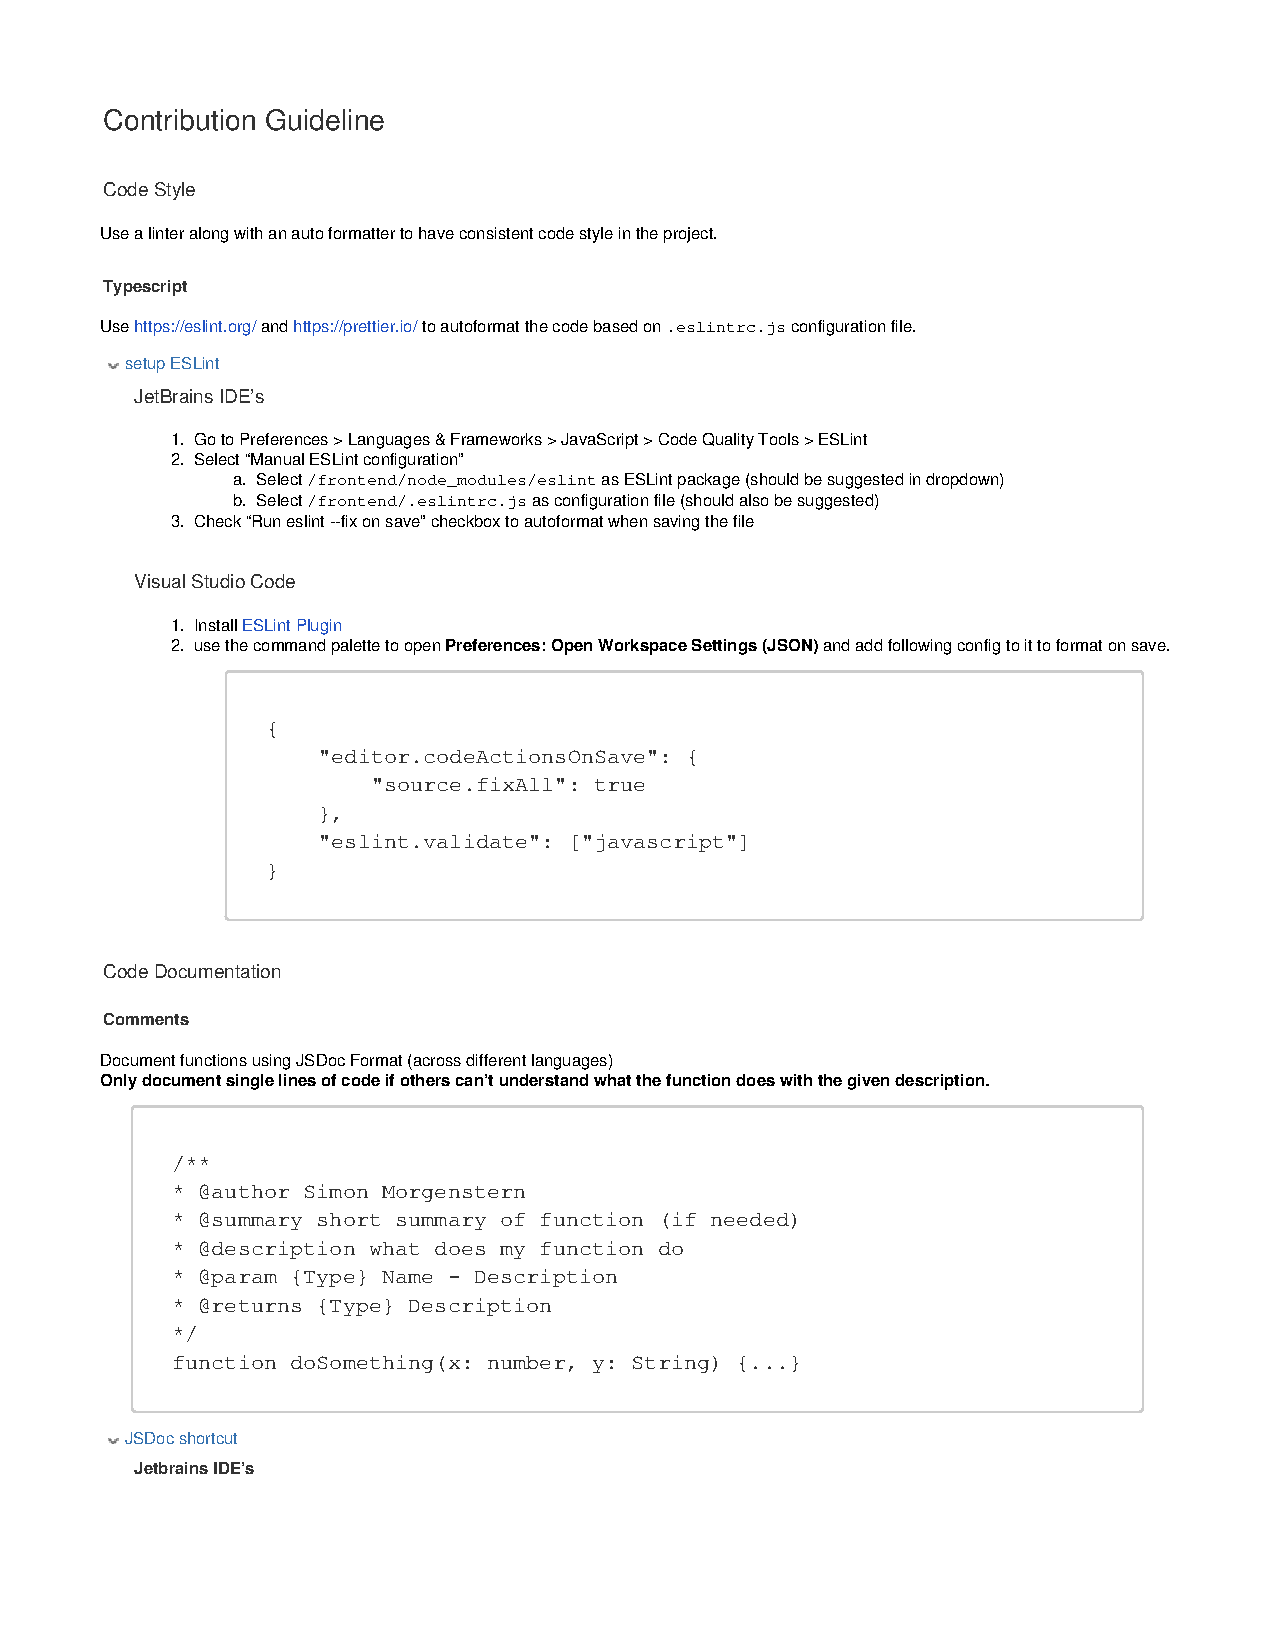
\includegraphics[width=\linewidth, page=1]{SKIOSA-ContributionGuideline.pdf}
    \caption*{Contribution Guideline - Seite 1}
\end{figure}
\begin{figure}[H]
    \includegraphics[width=\linewidth, page=2]{SKIOSA-ContributionGuideline.pdf}
    \caption*{figure}{Contribution Guideline - Seite 2}
\end{figure}

\subsection{Testing Guideline}
\begin{figure}[H]
    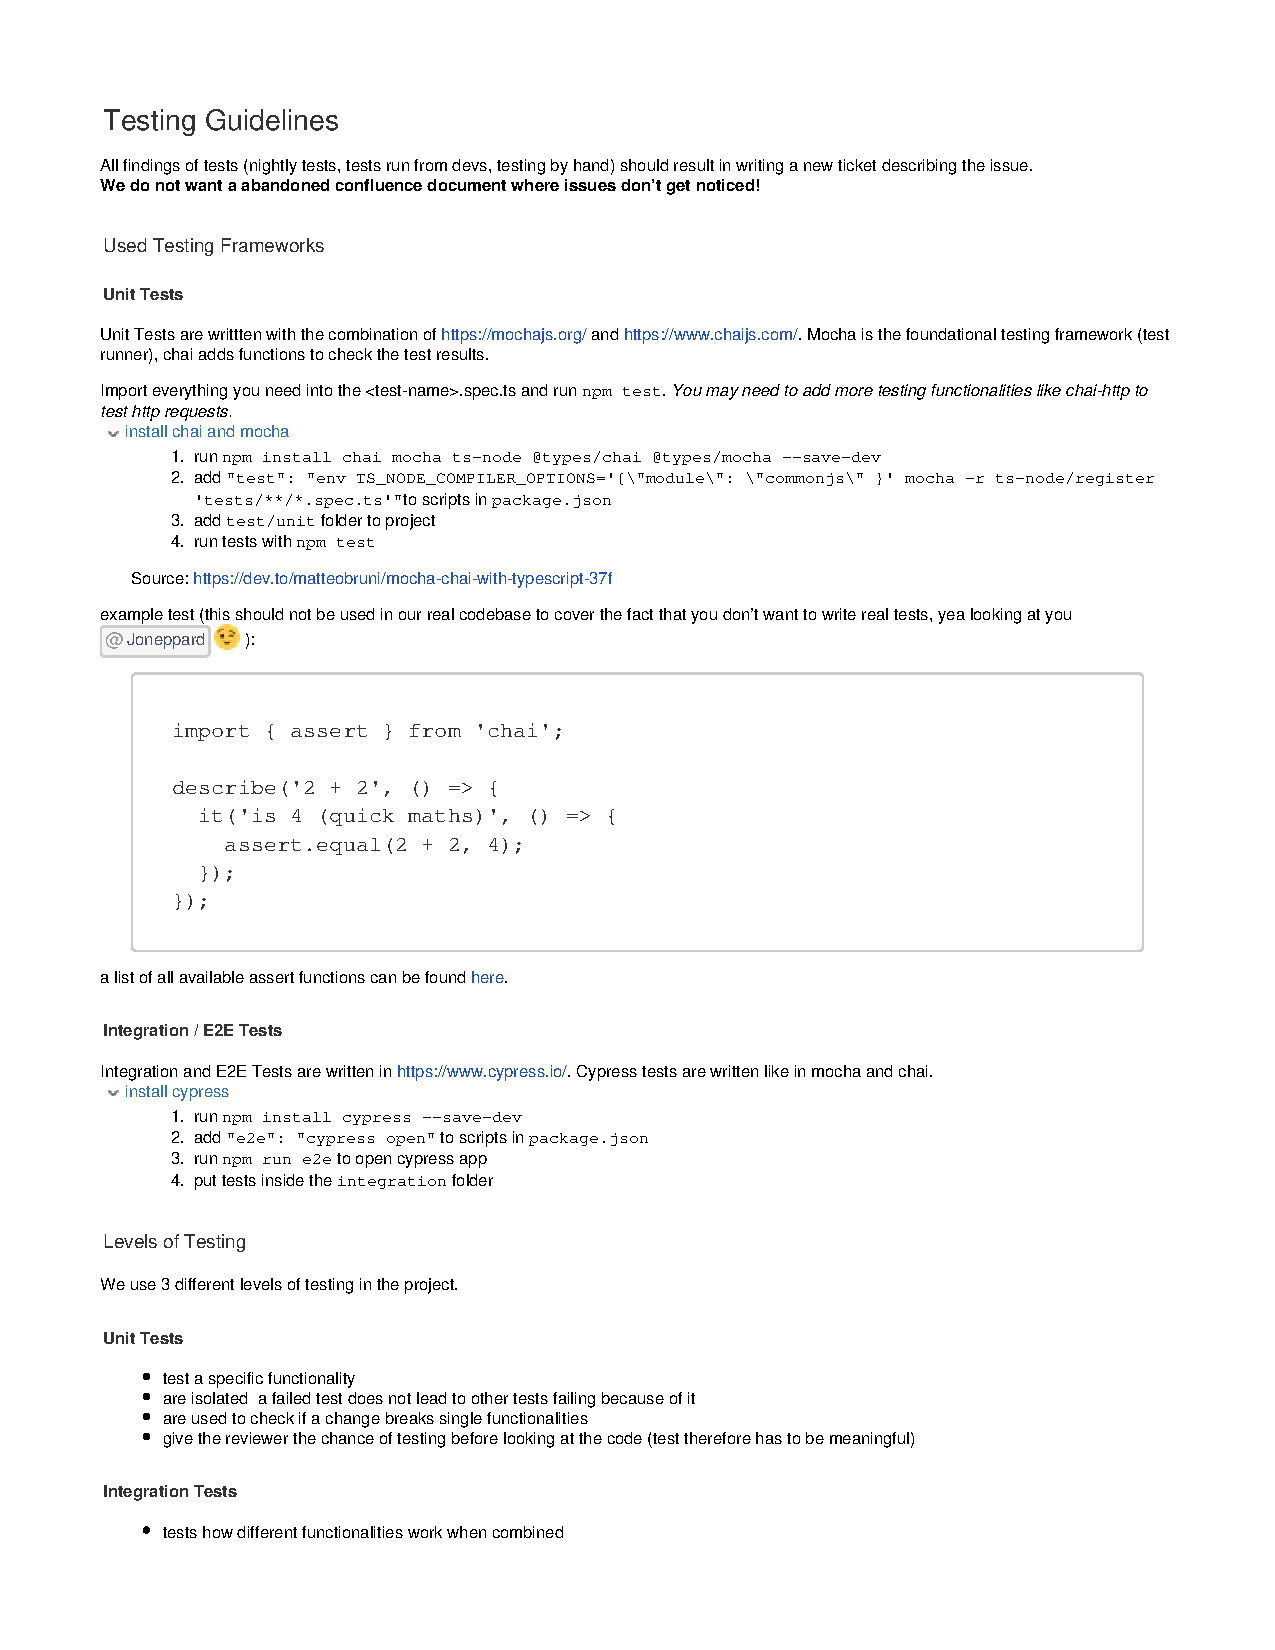
\includegraphics[width=\linewidth, page=1]{SKIOSA-TestingGuidelines.pdf}
    \caption*{Testing Guideline - Seite 1}
\end{figure}
\begin{figure}[H]
    \includegraphics[width=\linewidth, page=2]{SKIOSA-TestingGuidelines.pdf}
    \caption*{Testing Guideline - Seite 2}
\end{figure}

\section{Dokumentation der Software}
\subsection{Frontend}
\begin{figure}[H]
    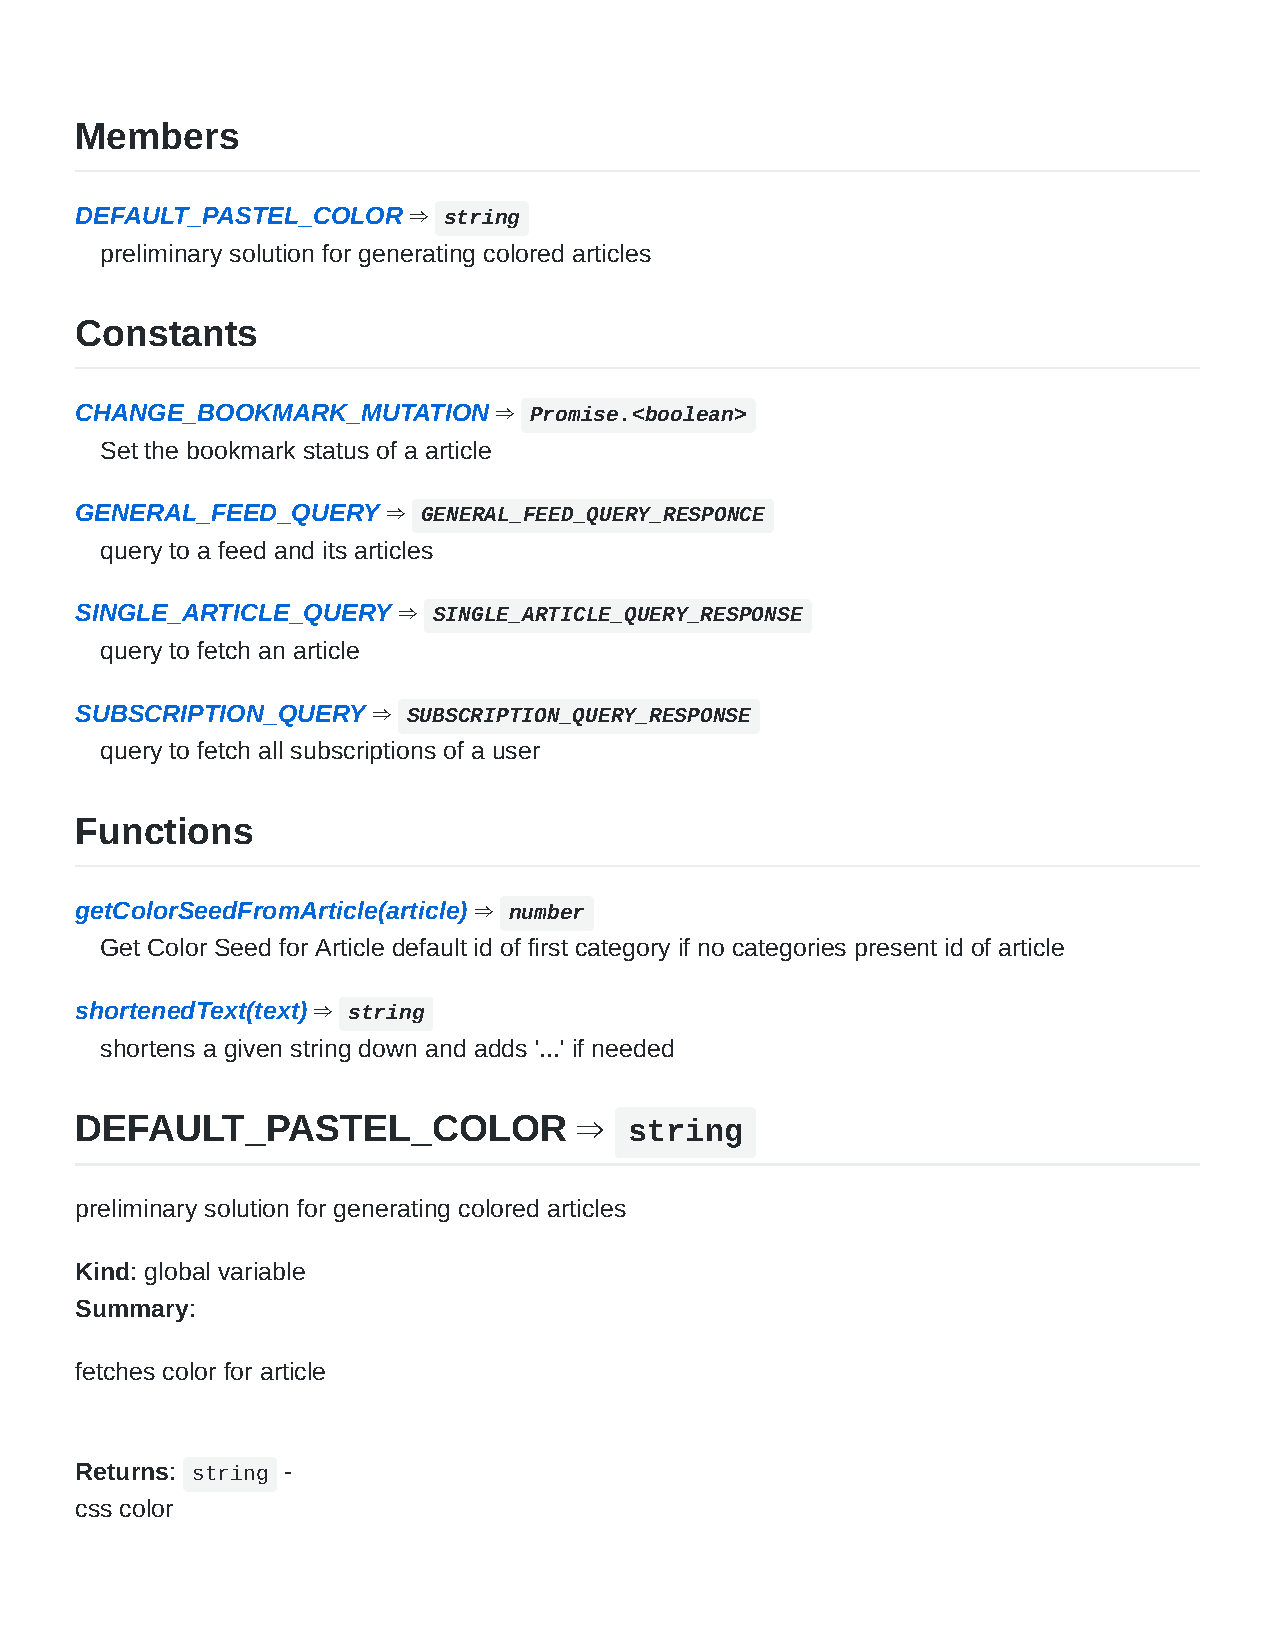
\includegraphics[width=\linewidth, page=1]{frontend.pdf}
    \caption*{Ausschnitt des Frontend JSDoc - Seite 1}
\end{figure}
\begin{figure}[H]
    \includegraphics[width=\linewidth, page=2]{frontend.pdf}
    \caption*{Ausschnitt des Frontend JSDoc - Seite 2}
\end{figure}
\begin{figure}[H]
    \includegraphics[width=\linewidth, page=3]{frontend.pdf}
    \caption*{Ausschnitt des Frontend JSDoc - Seite 3}
\end{figure}
\begin{figure}[H]
    \includegraphics[width=\linewidth, page=4]{frontend.pdf}
    \caption*{Ausschnitt des Frontend JSDoc - Seite 4}
\end{figure}
\begin{figure}[H]
    \includegraphics[width=\linewidth, page=5]{frontend.pdf}
    \caption*{Ausschnitt des Frontend JSDoc - Seite 5}
\end{figure}

\subsection{Core-Service}
\begin{figure}[H]
    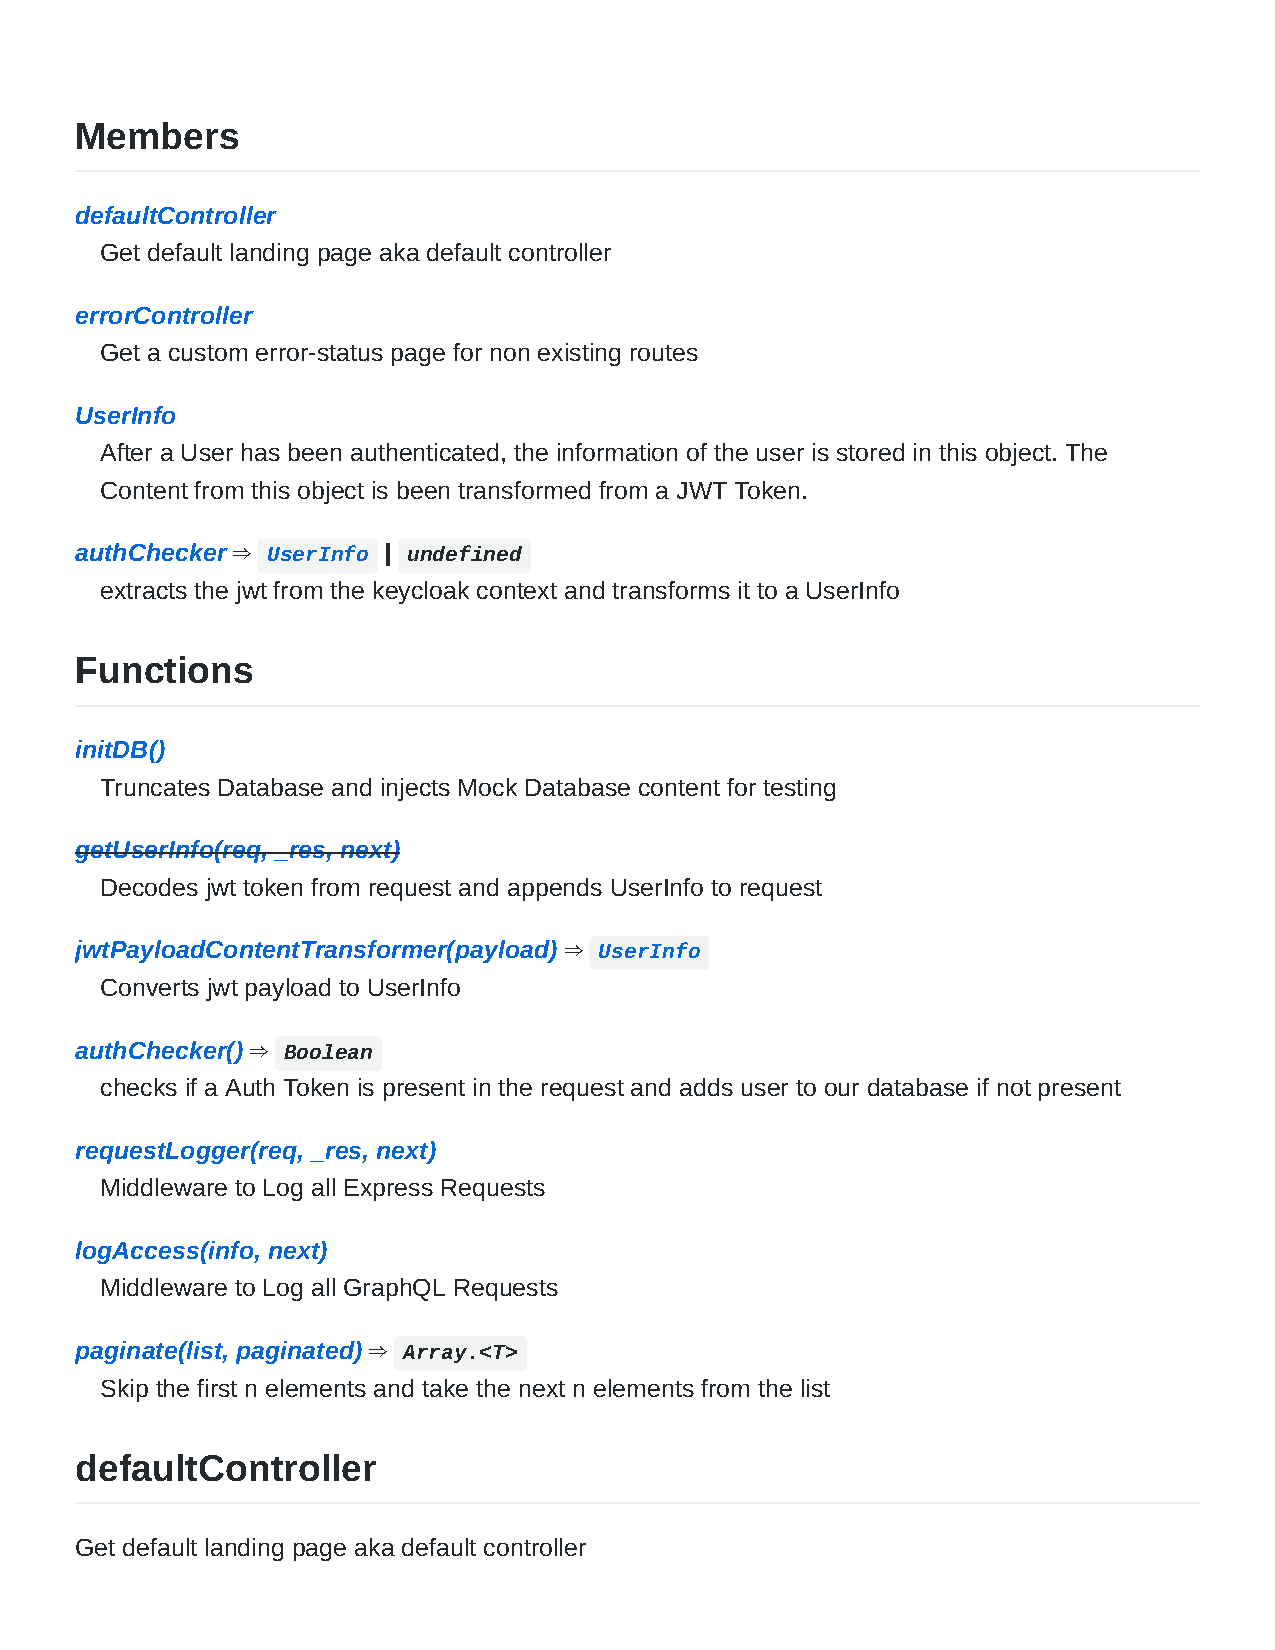
\includegraphics[width=\linewidth, page=1]{core_service_docs.pdf}
    \caption*{Ausschnitt des Core Service JSDoc - Seite 1}
\end{figure}
\begin{figure}[H]
    \includegraphics[width=\linewidth, page=2]{core_service_docs.pdf}
    \caption*{Ausschnitt des Core Service JSDoc - Seite 2}
\end{figure}
\begin{figure}[H]
    \includegraphics[width=\linewidth, page=3]{core_service_docs.pdf}
    \caption*{Ausschnitt des Core Service JSDoc - Seite 3}
\end{figure}
\begin{figure}[H]
    \includegraphics[width=\linewidth, page=4]{core_service_docs.pdf}
    \caption*{Ausschnitt des Core Service JSDoc - Seite 4}
\end{figure}
\begin{figure}[H]
    \includegraphics[width=\linewidth, page=5]{core_service_docs.pdf}
    \caption*{Ausschnitt des Core Service JSDoc - Seite 5}
\end{figure}
\begin{figure}[H]
    \includegraphics[width=\linewidth, page=6]{core_service_docs.pdf}
    \caption*{Ausschnitt des Core Service JSDoc - Seite 6}
\end{figure}

\subsection{Polling-Service}
\begin{figure}[H]
    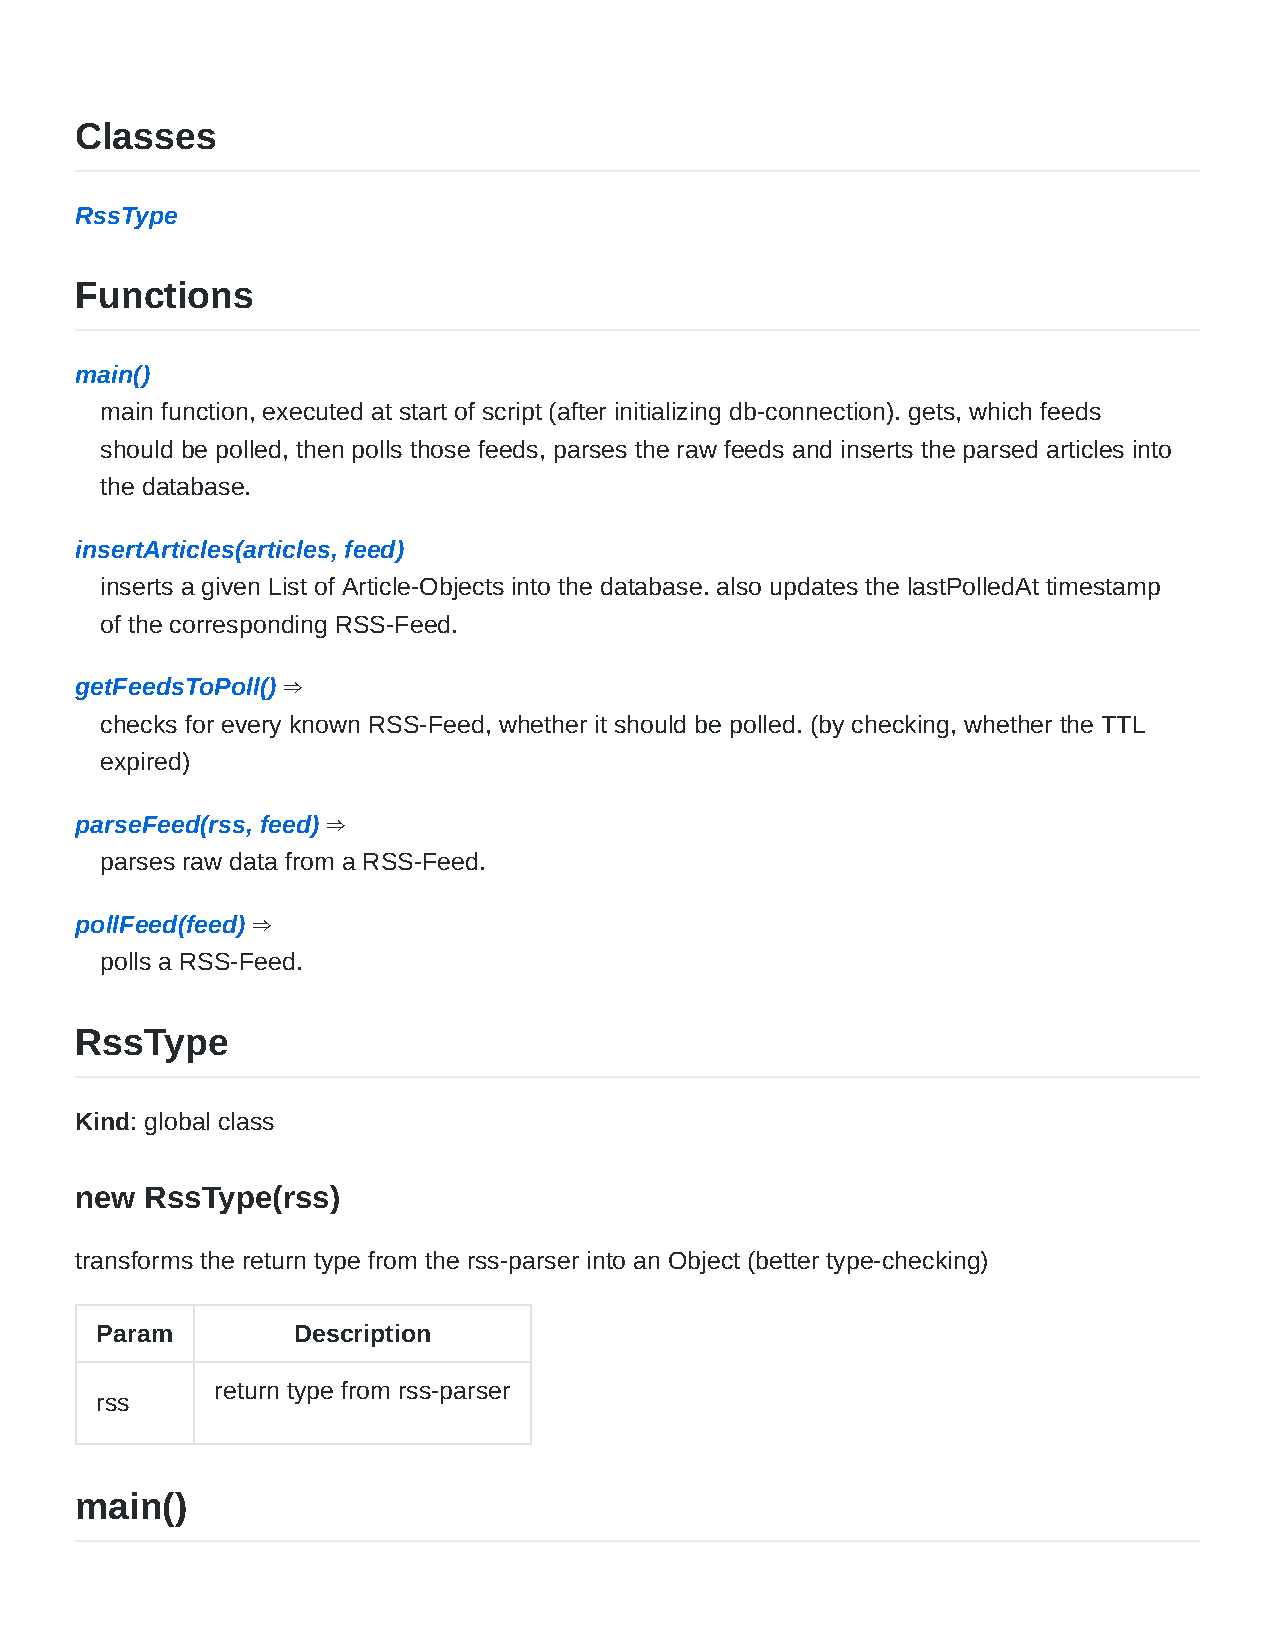
\includegraphics[width=\linewidth, page=1]{polling_service.pdf}
    \caption*{Ausschnitt des Polling Service JSDoc - Seite 1}
\end{figure}
\begin{figure}[H]
    \includegraphics[width=\linewidth, page=2]{polling_service.pdf}
    \caption*{Ausschnitt des Polling Service JSDoc - Seite 2}
\end{figure}
\begin{figure}[H]
    \includegraphics[width=\linewidth, page=3]{polling_service.pdf}
    \caption*{Ausschnitt des Polling Service JSDoc - Seite 3}
\end{figure}
\fi
\end{document}
